% Created by tikzDevice version 0.9 on 2016-01-11 22:38:27
% !TEX encoding = UTF-8 Unicode
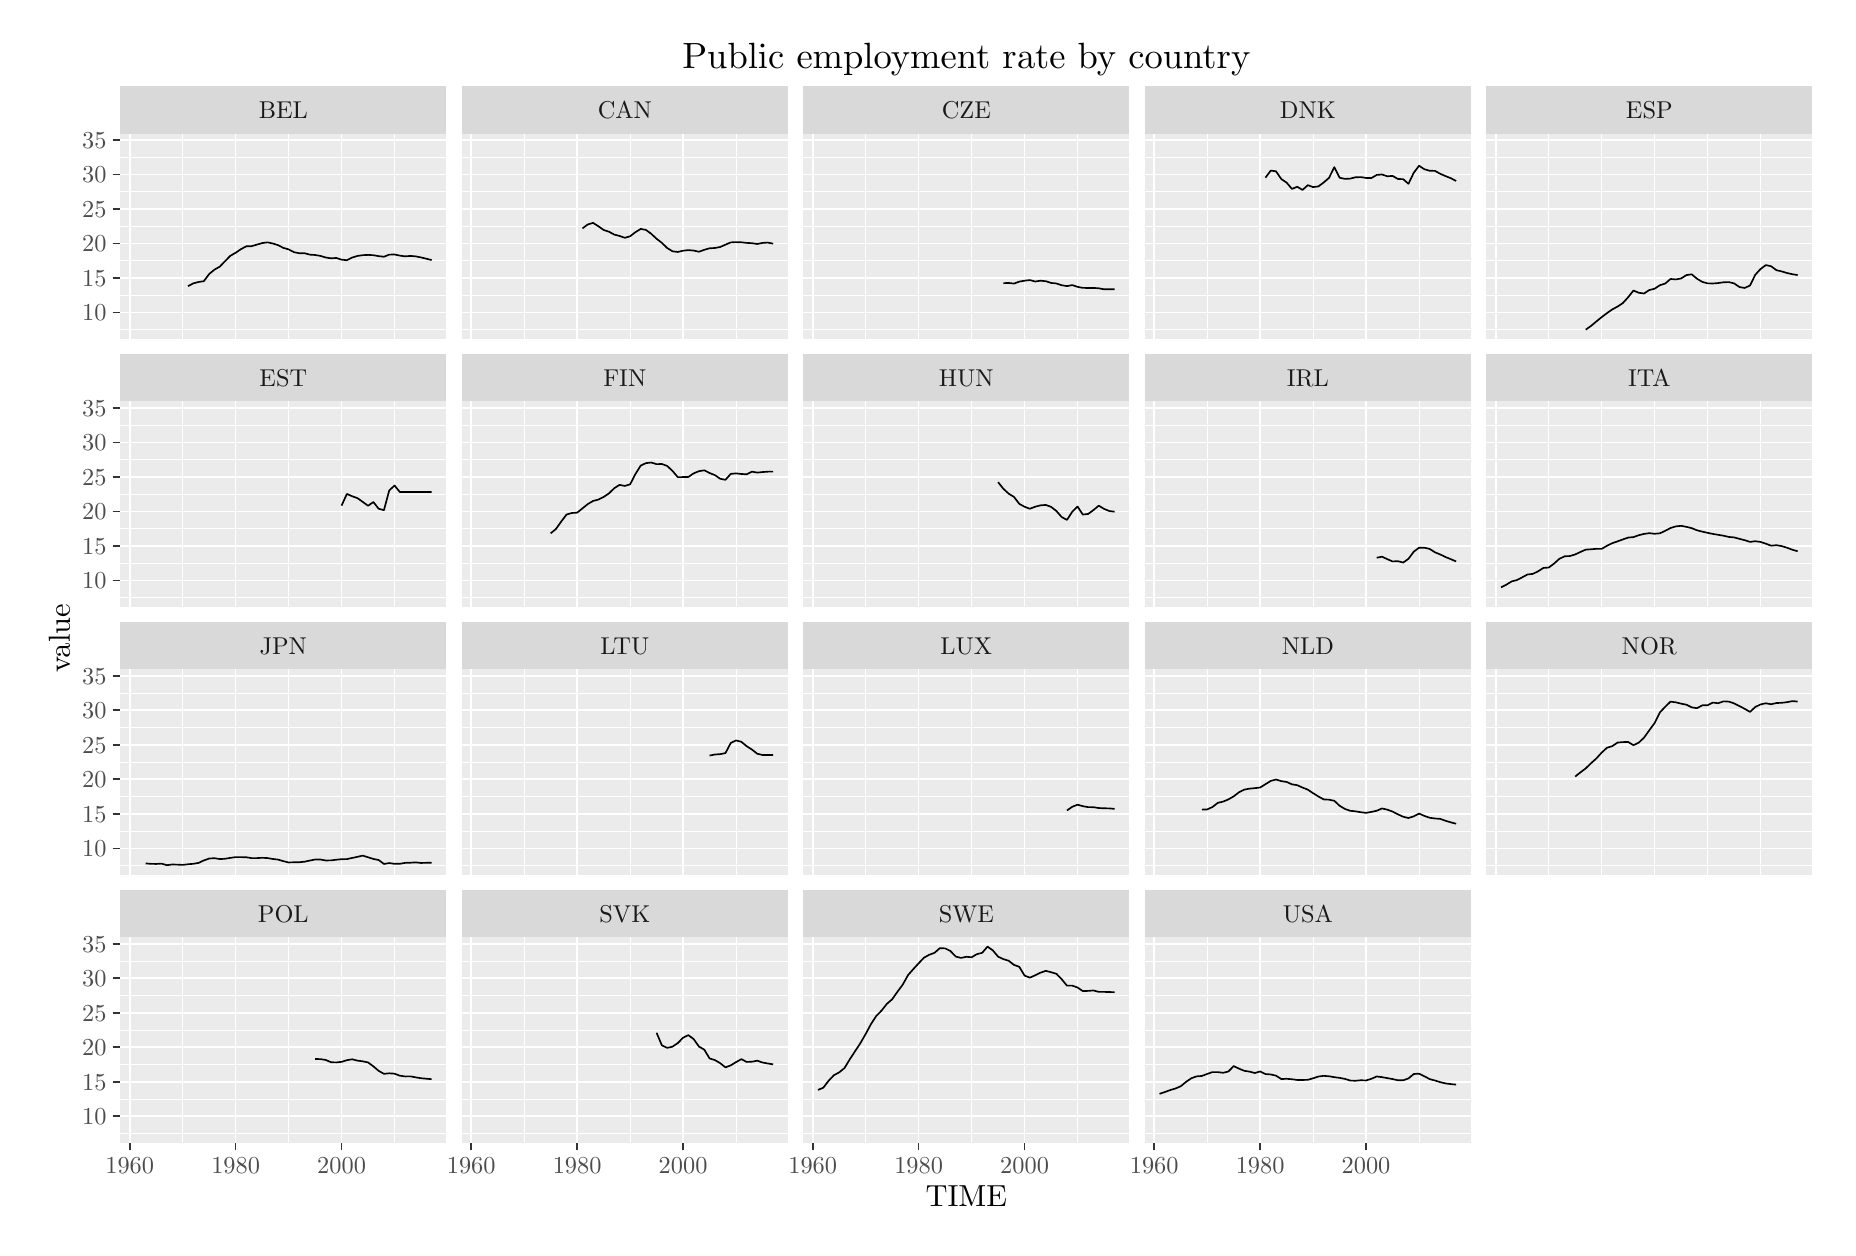
\begin{tikzpicture}[x=1pt,y=1pt]
\definecolor{fillColor}{RGB}{255,255,255}
\path[use as bounding box,fill=fillColor,fill opacity=0.00] (0,0) rectangle (650.43,433.62);
\begin{scope}
\path[clip] (  0.00,  0.00) rectangle (650.43,433.62);
\definecolor{drawColor}{RGB}{255,255,255}
\definecolor{fillColor}{RGB}{255,255,255}

\path[draw=drawColor,line width= 0.6pt,line join=round,line cap=round,fill=fillColor] (  0.00,  0.00) rectangle (650.43,433.62);
\end{scope}
\begin{scope}
\path[clip] ( 33.42,321.12) rectangle (151.33,395.37);
\definecolor{fillColor}{gray}{0.92}

\path[fill=fillColor] ( 33.42,321.12) rectangle (151.33,395.37);
\definecolor{drawColor}{RGB}{255,255,255}

\path[draw=drawColor,line width= 0.3pt,line join=round] ( 33.42,324.46) --
	(151.33,324.46);

\path[draw=drawColor,line width= 0.3pt,line join=round] ( 33.42,336.93) --
	(151.33,336.93);

\path[draw=drawColor,line width= 0.3pt,line join=round] ( 33.42,349.40) --
	(151.33,349.40);

\path[draw=drawColor,line width= 0.3pt,line join=round] ( 33.42,361.87) --
	(151.33,361.87);

\path[draw=drawColor,line width= 0.3pt,line join=round] ( 33.42,374.34) --
	(151.33,374.34);

\path[draw=drawColor,line width= 0.3pt,line join=round] ( 33.42,386.81) --
	(151.33,386.81);

\path[draw=drawColor,line width= 0.3pt,line join=round] ( 56.01,321.12) --
	( 56.01,395.37);

\path[draw=drawColor,line width= 0.3pt,line join=round] ( 94.29,321.12) --
	( 94.29,395.37);

\path[draw=drawColor,line width= 0.3pt,line join=round] (132.57,321.12) --
	(132.57,395.37);

\path[draw=drawColor,line width= 0.6pt,line join=round] ( 33.42,330.69) --
	(151.33,330.69);

\path[draw=drawColor,line width= 0.6pt,line join=round] ( 33.42,343.16) --
	(151.33,343.16);

\path[draw=drawColor,line width= 0.6pt,line join=round] ( 33.42,355.63) --
	(151.33,355.63);

\path[draw=drawColor,line width= 0.6pt,line join=round] ( 33.42,368.10) --
	(151.33,368.10);

\path[draw=drawColor,line width= 0.6pt,line join=round] ( 33.42,380.57) --
	(151.33,380.57);

\path[draw=drawColor,line width= 0.6pt,line join=round] ( 33.42,393.04) --
	(151.33,393.04);

\path[draw=drawColor,line width= 0.6pt,line join=round] ( 36.87,321.12) --
	( 36.87,395.37);

\path[draw=drawColor,line width= 0.6pt,line join=round] ( 75.15,321.12) --
	( 75.15,395.37);

\path[draw=drawColor,line width= 0.6pt,line join=round] (113.43,321.12) --
	(113.43,395.37);
\definecolor{drawColor}{RGB}{0,0,0}

\path[draw=drawColor,line width= 0.6pt,line join=round] ( 57.92,340.19) --
	( 59.84,341.22) --
	( 61.75,341.72) --
	( 63.66,342.01) --
	( 65.58,344.60) --
	( 67.49,346.18) --
	( 69.41,347.25) --
	( 71.32,349.24) --
	( 73.23,351.18) --
	( 75.15,352.28) --
	( 77.06,353.57) --
	( 78.98,354.61) --
	( 80.89,354.65) --
	( 82.80,355.21) --
	( 84.72,355.77) --
	( 86.63,356.05) --
	( 88.55,355.63) --
	( 90.46,355.04) --
	( 92.37,354.05) --
	( 94.29,353.51) --
	( 96.20,352.50) --
	( 98.12,352.11) --
	(100.03,352.12) --
	(101.94,351.60) --
	(103.86,351.47) --
	(105.77,351.15) --
	(107.69,350.57) --
	(109.60,350.27) --
	(111.51,350.40) --
	(113.43,349.79) --
	(115.34,349.59) --
	(117.26,350.55) --
	(119.17,351.14) --
	(121.08,351.41) --
	(123.00,351.51) --
	(124.91,351.40) --
	(126.83,351.06) --
	(128.74,350.85) --
	(130.65,351.60) --
	(132.57,351.66) --
	(134.48,351.24) --
	(136.40,350.98) --
	(138.31,351.14) --
	(140.22,350.97) --
	(142.14,350.59) --
	(144.05,350.13) --
	(145.97,349.64);
\end{scope}
\begin{scope}
\path[clip] (156.83,321.12) rectangle (274.73,395.37);
\definecolor{fillColor}{gray}{0.92}

\path[fill=fillColor] (156.83,321.12) rectangle (274.73,395.37);
\definecolor{drawColor}{RGB}{255,255,255}

\path[draw=drawColor,line width= 0.3pt,line join=round] (156.83,324.46) --
	(274.73,324.46);

\path[draw=drawColor,line width= 0.3pt,line join=round] (156.83,336.93) --
	(274.73,336.93);

\path[draw=drawColor,line width= 0.3pt,line join=round] (156.83,349.40) --
	(274.73,349.40);

\path[draw=drawColor,line width= 0.3pt,line join=round] (156.83,361.87) --
	(274.73,361.87);

\path[draw=drawColor,line width= 0.3pt,line join=round] (156.83,374.34) --
	(274.73,374.34);

\path[draw=drawColor,line width= 0.3pt,line join=round] (156.83,386.81) --
	(274.73,386.81);

\path[draw=drawColor,line width= 0.3pt,line join=round] (179.41,321.12) --
	(179.41,395.37);

\path[draw=drawColor,line width= 0.3pt,line join=round] (217.69,321.12) --
	(217.69,395.37);

\path[draw=drawColor,line width= 0.3pt,line join=round] (255.97,321.12) --
	(255.97,395.37);

\path[draw=drawColor,line width= 0.6pt,line join=round] (156.83,330.69) --
	(274.73,330.69);

\path[draw=drawColor,line width= 0.6pt,line join=round] (156.83,343.16) --
	(274.73,343.16);

\path[draw=drawColor,line width= 0.6pt,line join=round] (156.83,355.63) --
	(274.73,355.63);

\path[draw=drawColor,line width= 0.6pt,line join=round] (156.83,368.10) --
	(274.73,368.10);

\path[draw=drawColor,line width= 0.6pt,line join=round] (156.83,380.57) --
	(274.73,380.57);

\path[draw=drawColor,line width= 0.6pt,line join=round] (156.83,393.04) --
	(274.73,393.04);

\path[draw=drawColor,line width= 0.6pt,line join=round] (160.27,321.12) --
	(160.27,395.37);

\path[draw=drawColor,line width= 0.6pt,line join=round] (198.55,321.12) --
	(198.55,395.37);

\path[draw=drawColor,line width= 0.6pt,line join=round] (236.83,321.12) --
	(236.83,395.37);
\definecolor{drawColor}{RGB}{0,0,0}

\path[draw=drawColor,line width= 0.6pt,line join=round] (200.46,361.08) --
	(202.38,362.50) --
	(204.29,363.08) --
	(206.21,361.87) --
	(208.12,360.52) --
	(210.03,359.89) --
	(211.95,358.85) --
	(213.86,358.36) --
	(215.78,357.68) --
	(217.69,358.24) --
	(219.60,359.71) --
	(221.52,360.90) --
	(223.43,360.53) --
	(225.35,359.10) --
	(227.26,357.33) --
	(229.17,355.85) --
	(231.09,353.99) --
	(233.00,352.81) --
	(234.92,352.57) --
	(236.83,353.03) --
	(238.74,353.23) --
	(240.66,353.07) --
	(242.57,352.65) --
	(244.49,353.34) --
	(246.40,353.90) --
	(248.31,354.00) --
	(250.23,354.36) --
	(252.14,355.20) --
	(254.06,356.03) --
	(255.97,356.12) --
	(257.88,356.06) --
	(259.80,355.85) --
	(261.71,355.74) --
	(263.63,355.45) --
	(265.54,355.84) --
	(267.45,355.96) --
	(269.37,355.56);
\end{scope}
\begin{scope}
\path[clip] (280.23,321.12) rectangle (398.13,395.37);
\definecolor{fillColor}{gray}{0.92}

\path[fill=fillColor] (280.23,321.12) rectangle (398.13,395.37);
\definecolor{drawColor}{RGB}{255,255,255}

\path[draw=drawColor,line width= 0.3pt,line join=round] (280.23,324.46) --
	(398.13,324.46);

\path[draw=drawColor,line width= 0.3pt,line join=round] (280.23,336.93) --
	(398.13,336.93);

\path[draw=drawColor,line width= 0.3pt,line join=round] (280.23,349.40) --
	(398.13,349.40);

\path[draw=drawColor,line width= 0.3pt,line join=round] (280.23,361.87) --
	(398.13,361.87);

\path[draw=drawColor,line width= 0.3pt,line join=round] (280.23,374.34) --
	(398.13,374.34);

\path[draw=drawColor,line width= 0.3pt,line join=round] (280.23,386.81) --
	(398.13,386.81);

\path[draw=drawColor,line width= 0.3pt,line join=round] (302.81,321.12) --
	(302.81,395.37);

\path[draw=drawColor,line width= 0.3pt,line join=round] (341.09,321.12) --
	(341.09,395.37);

\path[draw=drawColor,line width= 0.3pt,line join=round] (379.37,321.12) --
	(379.37,395.37);

\path[draw=drawColor,line width= 0.6pt,line join=round] (280.23,330.69) --
	(398.13,330.69);

\path[draw=drawColor,line width= 0.6pt,line join=round] (280.23,343.16) --
	(398.13,343.16);

\path[draw=drawColor,line width= 0.6pt,line join=round] (280.23,355.63) --
	(398.13,355.63);

\path[draw=drawColor,line width= 0.6pt,line join=round] (280.23,368.10) --
	(398.13,368.10);

\path[draw=drawColor,line width= 0.6pt,line join=round] (280.23,380.57) --
	(398.13,380.57);

\path[draw=drawColor,line width= 0.6pt,line join=round] (280.23,393.04) --
	(398.13,393.04);

\path[draw=drawColor,line width= 0.6pt,line join=round] (283.67,321.12) --
	(283.67,395.37);

\path[draw=drawColor,line width= 0.6pt,line join=round] (321.95,321.12) --
	(321.95,395.37);

\path[draw=drawColor,line width= 0.6pt,line join=round] (360.23,321.12) --
	(360.23,395.37);
\definecolor{drawColor}{RGB}{0,0,0}

\path[draw=drawColor,line width= 0.6pt,line join=round] (352.57,341.28) --
	(354.49,341.38) --
	(356.40,341.14) --
	(358.32,341.86) --
	(360.23,342.19) --
	(362.14,342.41) --
	(364.06,341.89) --
	(365.97,342.18) --
	(367.89,342.00) --
	(369.80,341.36) --
	(371.71,341.20) --
	(373.63,340.55) --
	(375.54,340.23) --
	(377.46,340.60) --
	(379.37,339.96) --
	(381.28,339.58) --
	(383.20,339.57) --
	(385.11,339.57) --
	(387.03,339.44) --
	(388.94,339.08) --
	(390.85,339.08) --
	(392.77,339.08);
\end{scope}
\begin{scope}
\path[clip] (403.63,321.12) rectangle (521.53,395.37);
\definecolor{fillColor}{gray}{0.92}

\path[fill=fillColor] (403.63,321.12) rectangle (521.53,395.37);
\definecolor{drawColor}{RGB}{255,255,255}

\path[draw=drawColor,line width= 0.3pt,line join=round] (403.63,324.46) --
	(521.53,324.46);

\path[draw=drawColor,line width= 0.3pt,line join=round] (403.63,336.93) --
	(521.53,336.93);

\path[draw=drawColor,line width= 0.3pt,line join=round] (403.63,349.40) --
	(521.53,349.40);

\path[draw=drawColor,line width= 0.3pt,line join=round] (403.63,361.87) --
	(521.53,361.87);

\path[draw=drawColor,line width= 0.3pt,line join=round] (403.63,374.34) --
	(521.53,374.34);

\path[draw=drawColor,line width= 0.3pt,line join=round] (403.63,386.81) --
	(521.53,386.81);

\path[draw=drawColor,line width= 0.3pt,line join=round] (426.21,321.12) --
	(426.21,395.37);

\path[draw=drawColor,line width= 0.3pt,line join=round] (464.49,321.12) --
	(464.49,395.37);

\path[draw=drawColor,line width= 0.3pt,line join=round] (502.77,321.12) --
	(502.77,395.37);

\path[draw=drawColor,line width= 0.6pt,line join=round] (403.63,330.69) --
	(521.53,330.69);

\path[draw=drawColor,line width= 0.6pt,line join=round] (403.63,343.16) --
	(521.53,343.16);

\path[draw=drawColor,line width= 0.6pt,line join=round] (403.63,355.63) --
	(521.53,355.63);

\path[draw=drawColor,line width= 0.6pt,line join=round] (403.63,368.10) --
	(521.53,368.10);

\path[draw=drawColor,line width= 0.6pt,line join=round] (403.63,380.57) --
	(521.53,380.57);

\path[draw=drawColor,line width= 0.6pt,line join=round] (403.63,393.04) --
	(521.53,393.04);

\path[draw=drawColor,line width= 0.6pt,line join=round] (407.07,321.12) --
	(407.07,395.37);

\path[draw=drawColor,line width= 0.6pt,line join=round] (445.35,321.12) --
	(445.35,395.37);

\path[draw=drawColor,line width= 0.6pt,line join=round] (483.63,321.12) --
	(483.63,395.37);
\definecolor{drawColor}{RGB}{0,0,0}

\path[draw=drawColor,line width= 0.6pt,line join=round] (447.27,379.41) --
	(449.18,381.98) --
	(451.09,381.70) --
	(453.01,378.89) --
	(454.92,377.61) --
	(456.84,375.36) --
	(458.75,376.13) --
	(460.66,374.98) --
	(462.58,376.71) --
	(464.49,376.00) --
	(466.41,376.26) --
	(468.32,377.69) --
	(470.23,379.33) --
	(472.15,383.21) --
	(474.06,379.40) --
	(475.98,378.97) --
	(477.89,379.07) --
	(479.80,379.56) --
	(481.72,379.62) --
	(483.63,379.31) --
	(485.55,379.27) --
	(487.46,380.40) --
	(489.37,380.57) --
	(491.29,379.91) --
	(493.20,380.05) --
	(495.12,378.94) --
	(497.03,378.87) --
	(498.94,377.21) --
	(500.86,381.19) --
	(502.77,383.72) --
	(504.69,382.46) --
	(506.60,381.91) --
	(508.51,381.87) --
	(510.43,380.81) --
	(512.34,379.98) --
	(514.26,379.22) --
	(516.17,378.23);
\end{scope}
\begin{scope}
\path[clip] (527.03,321.12) rectangle (644.93,395.37);
\definecolor{fillColor}{gray}{0.92}

\path[fill=fillColor] (527.03,321.12) rectangle (644.93,395.37);
\definecolor{drawColor}{RGB}{255,255,255}

\path[draw=drawColor,line width= 0.3pt,line join=round] (527.03,324.46) --
	(644.93,324.46);

\path[draw=drawColor,line width= 0.3pt,line join=round] (527.03,336.93) --
	(644.93,336.93);

\path[draw=drawColor,line width= 0.3pt,line join=round] (527.03,349.40) --
	(644.93,349.40);

\path[draw=drawColor,line width= 0.3pt,line join=round] (527.03,361.87) --
	(644.93,361.87);

\path[draw=drawColor,line width= 0.3pt,line join=round] (527.03,374.34) --
	(644.93,374.34);

\path[draw=drawColor,line width= 0.3pt,line join=round] (527.03,386.81) --
	(644.93,386.81);

\path[draw=drawColor,line width= 0.3pt,line join=round] (549.61,321.12) --
	(549.61,395.37);

\path[draw=drawColor,line width= 0.3pt,line join=round] (587.89,321.12) --
	(587.89,395.37);

\path[draw=drawColor,line width= 0.3pt,line join=round] (626.17,321.12) --
	(626.17,395.37);

\path[draw=drawColor,line width= 0.6pt,line join=round] (527.03,330.69) --
	(644.93,330.69);

\path[draw=drawColor,line width= 0.6pt,line join=round] (527.03,343.16) --
	(644.93,343.16);

\path[draw=drawColor,line width= 0.6pt,line join=round] (527.03,355.63) --
	(644.93,355.63);

\path[draw=drawColor,line width= 0.6pt,line join=round] (527.03,368.10) --
	(644.93,368.10);

\path[draw=drawColor,line width= 0.6pt,line join=round] (527.03,380.57) --
	(644.93,380.57);

\path[draw=drawColor,line width= 0.6pt,line join=round] (527.03,393.04) --
	(644.93,393.04);

\path[draw=drawColor,line width= 0.6pt,line join=round] (530.47,321.12) --
	(530.47,395.37);

\path[draw=drawColor,line width= 0.6pt,line join=round] (568.75,321.12) --
	(568.75,395.37);

\path[draw=drawColor,line width= 0.6pt,line join=round] (607.03,321.12) --
	(607.03,395.37);
\definecolor{drawColor}{RGB}{0,0,0}

\path[draw=drawColor,line width= 0.6pt,line join=round] (563.01,324.49) --
	(564.93,325.86) --
	(566.84,327.46) --
	(568.75,329.02) --
	(570.67,330.47) --
	(572.58,331.80) --
	(574.50,332.84) --
	(576.41,334.10) --
	(578.32,336.21) --
	(580.24,338.63) --
	(582.15,337.83) --
	(584.07,337.56) --
	(585.98,338.82) --
	(587.89,339.28) --
	(589.81,340.56) --
	(591.72,341.15) --
	(593.64,342.81) --
	(595.55,342.64) --
	(597.46,342.99) --
	(599.38,344.22) --
	(601.29,344.49) --
	(603.21,342.89) --
	(605.12,341.75) --
	(607.03,341.23) --
	(608.95,341.18) --
	(610.86,341.33) --
	(612.78,341.61) --
	(614.69,341.68) --
	(616.60,341.22) --
	(618.52,339.90) --
	(620.43,339.56) --
	(622.35,340.43) --
	(624.26,344.33) --
	(626.17,346.41) --
	(628.09,347.83) --
	(630.00,347.40) --
	(631.91,345.98) --
	(633.83,345.54) --
	(635.74,344.96) --
	(637.66,344.53) --
	(639.57,344.22);
\end{scope}
\begin{scope}
\path[clip] ( 33.42,224.31) rectangle (151.33,298.56);
\definecolor{fillColor}{gray}{0.92}

\path[fill=fillColor] ( 33.42,224.31) rectangle (151.33,298.56);
\definecolor{drawColor}{RGB}{255,255,255}

\path[draw=drawColor,line width= 0.3pt,line join=round] ( 33.42,227.65) --
	(151.33,227.65);

\path[draw=drawColor,line width= 0.3pt,line join=round] ( 33.42,240.12) --
	(151.33,240.12);

\path[draw=drawColor,line width= 0.3pt,line join=round] ( 33.42,252.59) --
	(151.33,252.59);

\path[draw=drawColor,line width= 0.3pt,line join=round] ( 33.42,265.06) --
	(151.33,265.06);

\path[draw=drawColor,line width= 0.3pt,line join=round] ( 33.42,277.53) --
	(151.33,277.53);

\path[draw=drawColor,line width= 0.3pt,line join=round] ( 33.42,290.00) --
	(151.33,290.00);

\path[draw=drawColor,line width= 0.3pt,line join=round] ( 56.01,224.31) --
	( 56.01,298.56);

\path[draw=drawColor,line width= 0.3pt,line join=round] ( 94.29,224.31) --
	( 94.29,298.56);

\path[draw=drawColor,line width= 0.3pt,line join=round] (132.57,224.31) --
	(132.57,298.56);

\path[draw=drawColor,line width= 0.6pt,line join=round] ( 33.42,233.88) --
	(151.33,233.88);

\path[draw=drawColor,line width= 0.6pt,line join=round] ( 33.42,246.35) --
	(151.33,246.35);

\path[draw=drawColor,line width= 0.6pt,line join=round] ( 33.42,258.82) --
	(151.33,258.82);

\path[draw=drawColor,line width= 0.6pt,line join=round] ( 33.42,271.29) --
	(151.33,271.29);

\path[draw=drawColor,line width= 0.6pt,line join=round] ( 33.42,283.76) --
	(151.33,283.76);

\path[draw=drawColor,line width= 0.6pt,line join=round] ( 33.42,296.23) --
	(151.33,296.23);

\path[draw=drawColor,line width= 0.6pt,line join=round] ( 36.87,224.31) --
	( 36.87,298.56);

\path[draw=drawColor,line width= 0.6pt,line join=round] ( 75.15,224.31) --
	( 75.15,298.56);

\path[draw=drawColor,line width= 0.6pt,line join=round] (113.43,224.31) --
	(113.43,298.56);
\definecolor{drawColor}{RGB}{0,0,0}

\path[draw=drawColor,line width= 0.6pt,line join=round] (113.43,260.92) --
	(115.34,265.13) --
	(117.26,264.30) --
	(119.17,263.61) --
	(121.08,262.26) --
	(123.00,260.85) --
	(124.91,262.21) --
	(126.83,259.78) --
	(128.74,259.27) --
	(130.65,266.40) --
	(132.57,268.17) --
	(134.48,265.82) --
	(136.40,265.82) --
	(138.31,265.82) --
	(140.22,265.82) --
	(142.14,265.82) --
	(144.05,265.82) --
	(145.97,265.82);
\end{scope}
\begin{scope}
\path[clip] (156.83,224.31) rectangle (274.73,298.56);
\definecolor{fillColor}{gray}{0.92}

\path[fill=fillColor] (156.83,224.31) rectangle (274.73,298.56);
\definecolor{drawColor}{RGB}{255,255,255}

\path[draw=drawColor,line width= 0.3pt,line join=round] (156.83,227.65) --
	(274.73,227.65);

\path[draw=drawColor,line width= 0.3pt,line join=round] (156.83,240.12) --
	(274.73,240.12);

\path[draw=drawColor,line width= 0.3pt,line join=round] (156.83,252.59) --
	(274.73,252.59);

\path[draw=drawColor,line width= 0.3pt,line join=round] (156.83,265.06) --
	(274.73,265.06);

\path[draw=drawColor,line width= 0.3pt,line join=round] (156.83,277.53) --
	(274.73,277.53);

\path[draw=drawColor,line width= 0.3pt,line join=round] (156.83,290.00) --
	(274.73,290.00);

\path[draw=drawColor,line width= 0.3pt,line join=round] (179.41,224.31) --
	(179.41,298.56);

\path[draw=drawColor,line width= 0.3pt,line join=round] (217.69,224.31) --
	(217.69,298.56);

\path[draw=drawColor,line width= 0.3pt,line join=round] (255.97,224.31) --
	(255.97,298.56);

\path[draw=drawColor,line width= 0.6pt,line join=round] (156.83,233.88) --
	(274.73,233.88);

\path[draw=drawColor,line width= 0.6pt,line join=round] (156.83,246.35) --
	(274.73,246.35);

\path[draw=drawColor,line width= 0.6pt,line join=round] (156.83,258.82) --
	(274.73,258.82);

\path[draw=drawColor,line width= 0.6pt,line join=round] (156.83,271.29) --
	(274.73,271.29);

\path[draw=drawColor,line width= 0.6pt,line join=round] (156.83,283.76) --
	(274.73,283.76);

\path[draw=drawColor,line width= 0.6pt,line join=round] (156.83,296.23) --
	(274.73,296.23);

\path[draw=drawColor,line width= 0.6pt,line join=round] (160.27,224.31) --
	(160.27,298.56);

\path[draw=drawColor,line width= 0.6pt,line join=round] (198.55,224.31) --
	(198.55,298.56);

\path[draw=drawColor,line width= 0.6pt,line join=round] (236.83,224.31) --
	(236.83,298.56);
\definecolor{drawColor}{RGB}{0,0,0}

\path[draw=drawColor,line width= 0.6pt,line join=round] (188.98,250.89) --
	(190.89,252.47) --
	(192.81,255.17) --
	(194.72,257.70) --
	(196.64,258.25) --
	(198.55,258.37) --
	(200.46,259.90) --
	(202.38,261.45) --
	(204.29,262.59) --
	(206.21,263.09) --
	(208.12,264.05) --
	(210.03,265.32) --
	(211.95,267.19) --
	(213.86,268.41) --
	(215.78,268.02) --
	(217.69,268.60) --
	(219.60,272.31) --
	(221.52,275.38) --
	(223.43,276.27) --
	(225.35,276.48) --
	(227.26,275.89) --
	(229.17,275.96) --
	(231.09,275.24) --
	(233.00,273.46) --
	(234.92,271.19) --
	(236.83,271.23) --
	(238.74,271.27) --
	(240.66,272.57) --
	(242.57,273.36) --
	(244.49,273.67) --
	(246.40,272.70) --
	(248.31,271.94) --
	(250.23,270.62) --
	(252.14,270.24) --
	(254.06,272.38) --
	(255.97,272.56) --
	(257.88,272.35) --
	(259.80,272.21) --
	(261.71,273.18) --
	(263.63,272.84) --
	(265.54,273.04) --
	(267.45,273.18) --
	(269.37,273.18);
\end{scope}
\begin{scope}
\path[clip] (280.23,224.31) rectangle (398.13,298.56);
\definecolor{fillColor}{gray}{0.92}

\path[fill=fillColor] (280.23,224.31) rectangle (398.13,298.56);
\definecolor{drawColor}{RGB}{255,255,255}

\path[draw=drawColor,line width= 0.3pt,line join=round] (280.23,227.65) --
	(398.13,227.65);

\path[draw=drawColor,line width= 0.3pt,line join=round] (280.23,240.12) --
	(398.13,240.12);

\path[draw=drawColor,line width= 0.3pt,line join=round] (280.23,252.59) --
	(398.13,252.59);

\path[draw=drawColor,line width= 0.3pt,line join=round] (280.23,265.06) --
	(398.13,265.06);

\path[draw=drawColor,line width= 0.3pt,line join=round] (280.23,277.53) --
	(398.13,277.53);

\path[draw=drawColor,line width= 0.3pt,line join=round] (280.23,290.00) --
	(398.13,290.00);

\path[draw=drawColor,line width= 0.3pt,line join=round] (302.81,224.31) --
	(302.81,298.56);

\path[draw=drawColor,line width= 0.3pt,line join=round] (341.09,224.31) --
	(341.09,298.56);

\path[draw=drawColor,line width= 0.3pt,line join=round] (379.37,224.31) --
	(379.37,298.56);

\path[draw=drawColor,line width= 0.6pt,line join=round] (280.23,233.88) --
	(398.13,233.88);

\path[draw=drawColor,line width= 0.6pt,line join=round] (280.23,246.35) --
	(398.13,246.35);

\path[draw=drawColor,line width= 0.6pt,line join=round] (280.23,258.82) --
	(398.13,258.82);

\path[draw=drawColor,line width= 0.6pt,line join=round] (280.23,271.29) --
	(398.13,271.29);

\path[draw=drawColor,line width= 0.6pt,line join=round] (280.23,283.76) --
	(398.13,283.76);

\path[draw=drawColor,line width= 0.6pt,line join=round] (280.23,296.23) --
	(398.13,296.23);

\path[draw=drawColor,line width= 0.6pt,line join=round] (283.67,224.31) --
	(283.67,298.56);

\path[draw=drawColor,line width= 0.6pt,line join=round] (321.95,224.31) --
	(321.95,298.56);

\path[draw=drawColor,line width= 0.6pt,line join=round] (360.23,224.31) --
	(360.23,298.56);
\definecolor{drawColor}{RGB}{0,0,0}

\path[draw=drawColor,line width= 0.6pt,line join=round] (350.66,269.37) --
	(352.57,266.99) --
	(354.49,265.22) --
	(356.40,264.06) --
	(358.32,261.54) --
	(360.23,260.49) --
	(362.14,259.78) --
	(364.06,260.51) --
	(365.97,261.01) --
	(367.89,261.16) --
	(369.80,260.46) --
	(371.71,258.99) --
	(373.63,256.79) --
	(375.54,255.74) --
	(377.46,258.71) --
	(379.37,260.57) --
	(381.28,257.68) --
	(383.20,257.90) --
	(385.11,259.30) --
	(387.03,260.89) --
	(388.94,259.74) --
	(390.85,258.95) --
	(392.77,258.71);
\end{scope}
\begin{scope}
\path[clip] (403.63,224.31) rectangle (521.53,298.56);
\definecolor{fillColor}{gray}{0.92}

\path[fill=fillColor] (403.63,224.31) rectangle (521.53,298.56);
\definecolor{drawColor}{RGB}{255,255,255}

\path[draw=drawColor,line width= 0.3pt,line join=round] (403.63,227.65) --
	(521.53,227.65);

\path[draw=drawColor,line width= 0.3pt,line join=round] (403.63,240.12) --
	(521.53,240.12);

\path[draw=drawColor,line width= 0.3pt,line join=round] (403.63,252.59) --
	(521.53,252.59);

\path[draw=drawColor,line width= 0.3pt,line join=round] (403.63,265.06) --
	(521.53,265.06);

\path[draw=drawColor,line width= 0.3pt,line join=round] (403.63,277.53) --
	(521.53,277.53);

\path[draw=drawColor,line width= 0.3pt,line join=round] (403.63,290.00) --
	(521.53,290.00);

\path[draw=drawColor,line width= 0.3pt,line join=round] (426.21,224.31) --
	(426.21,298.56);

\path[draw=drawColor,line width= 0.3pt,line join=round] (464.49,224.31) --
	(464.49,298.56);

\path[draw=drawColor,line width= 0.3pt,line join=round] (502.77,224.31) --
	(502.77,298.56);

\path[draw=drawColor,line width= 0.6pt,line join=round] (403.63,233.88) --
	(521.53,233.88);

\path[draw=drawColor,line width= 0.6pt,line join=round] (403.63,246.35) --
	(521.53,246.35);

\path[draw=drawColor,line width= 0.6pt,line join=round] (403.63,258.82) --
	(521.53,258.82);

\path[draw=drawColor,line width= 0.6pt,line join=round] (403.63,271.29) --
	(521.53,271.29);

\path[draw=drawColor,line width= 0.6pt,line join=round] (403.63,283.76) --
	(521.53,283.76);

\path[draw=drawColor,line width= 0.6pt,line join=round] (403.63,296.23) --
	(521.53,296.23);

\path[draw=drawColor,line width= 0.6pt,line join=round] (407.07,224.31) --
	(407.07,298.56);

\path[draw=drawColor,line width= 0.6pt,line join=round] (445.35,224.31) --
	(445.35,298.56);

\path[draw=drawColor,line width= 0.6pt,line join=round] (483.63,224.31) --
	(483.63,298.56);
\definecolor{drawColor}{RGB}{0,0,0}

\path[draw=drawColor,line width= 0.6pt,line join=round] (487.46,242.07) --
	(489.37,242.46) --
	(491.29,241.57) --
	(493.20,240.74) --
	(495.12,240.84) --
	(497.03,240.34) --
	(498.94,241.68) --
	(500.86,244.27) --
	(502.77,245.71) --
	(504.69,245.71) --
	(506.60,245.27) --
	(508.51,244.04) --
	(510.43,243.26) --
	(512.34,242.34) --
	(514.26,241.55) --
	(516.17,240.74);
\end{scope}
\begin{scope}
\path[clip] (527.03,224.31) rectangle (644.93,298.56);
\definecolor{fillColor}{gray}{0.92}

\path[fill=fillColor] (527.03,224.31) rectangle (644.93,298.56);
\definecolor{drawColor}{RGB}{255,255,255}

\path[draw=drawColor,line width= 0.3pt,line join=round] (527.03,227.65) --
	(644.93,227.65);

\path[draw=drawColor,line width= 0.3pt,line join=round] (527.03,240.12) --
	(644.93,240.12);

\path[draw=drawColor,line width= 0.3pt,line join=round] (527.03,252.59) --
	(644.93,252.59);

\path[draw=drawColor,line width= 0.3pt,line join=round] (527.03,265.06) --
	(644.93,265.06);

\path[draw=drawColor,line width= 0.3pt,line join=round] (527.03,277.53) --
	(644.93,277.53);

\path[draw=drawColor,line width= 0.3pt,line join=round] (527.03,290.00) --
	(644.93,290.00);

\path[draw=drawColor,line width= 0.3pt,line join=round] (549.61,224.31) --
	(549.61,298.56);

\path[draw=drawColor,line width= 0.3pt,line join=round] (587.89,224.31) --
	(587.89,298.56);

\path[draw=drawColor,line width= 0.3pt,line join=round] (626.17,224.31) --
	(626.17,298.56);

\path[draw=drawColor,line width= 0.6pt,line join=round] (527.03,233.88) --
	(644.93,233.88);

\path[draw=drawColor,line width= 0.6pt,line join=round] (527.03,246.35) --
	(644.93,246.35);

\path[draw=drawColor,line width= 0.6pt,line join=round] (527.03,258.82) --
	(644.93,258.82);

\path[draw=drawColor,line width= 0.6pt,line join=round] (527.03,271.29) --
	(644.93,271.29);

\path[draw=drawColor,line width= 0.6pt,line join=round] (527.03,283.76) --
	(644.93,283.76);

\path[draw=drawColor,line width= 0.6pt,line join=round] (527.03,296.23) --
	(644.93,296.23);

\path[draw=drawColor,line width= 0.6pt,line join=round] (530.47,224.31) --
	(530.47,298.56);

\path[draw=drawColor,line width= 0.6pt,line join=round] (568.75,224.31) --
	(568.75,298.56);

\path[draw=drawColor,line width= 0.6pt,line join=round] (607.03,224.31) --
	(607.03,298.56);
\definecolor{drawColor}{RGB}{0,0,0}

\path[draw=drawColor,line width= 0.6pt,line join=round] (532.39,231.38) --
	(534.30,232.34) --
	(536.22,233.52) --
	(538.13,234.00) --
	(540.04,234.99) --
	(541.96,236.03) --
	(543.87,236.24) --
	(545.79,237.18) --
	(547.70,238.39) --
	(549.61,238.53) --
	(551.53,239.94) --
	(553.44,241.66) --
	(555.36,242.60) --
	(557.27,242.69) --
	(559.18,243.27) --
	(561.10,244.17) --
	(563.01,245.01) --
	(564.93,245.13) --
	(566.84,245.30) --
	(568.75,245.28) --
	(570.67,246.40) --
	(572.58,247.33) --
	(574.50,248.00) --
	(576.41,248.69) --
	(578.32,249.36) --
	(580.24,249.53) --
	(582.15,250.22) --
	(584.07,250.69) --
	(585.98,250.96) --
	(587.89,250.74) --
	(589.81,250.91) --
	(591.72,251.80) --
	(593.64,252.82) --
	(595.55,253.40) --
	(597.46,253.61) --
	(599.38,253.24) --
	(601.29,252.77) --
	(603.21,252.00) --
	(605.12,251.51) --
	(607.03,251.08) --
	(608.95,250.69) --
	(610.86,250.36) --
	(612.78,250.04) --
	(614.69,249.59) --
	(616.60,249.43) --
	(618.52,248.91) --
	(620.43,248.43) --
	(622.35,247.80) --
	(624.26,248.04) --
	(626.17,247.79) --
	(628.09,247.15) --
	(630.00,246.43) --
	(631.91,246.61) --
	(633.83,246.28) --
	(635.74,245.68) --
	(637.66,244.98) --
	(639.57,244.41);
\end{scope}
\begin{scope}
\path[clip] ( 33.42,127.50) rectangle (151.33,201.75);
\definecolor{fillColor}{gray}{0.92}

\path[fill=fillColor] ( 33.42,127.50) rectangle (151.33,201.75);
\definecolor{drawColor}{RGB}{255,255,255}

\path[draw=drawColor,line width= 0.3pt,line join=round] ( 33.42,130.84) --
	(151.33,130.84);

\path[draw=drawColor,line width= 0.3pt,line join=round] ( 33.42,143.31) --
	(151.33,143.31);

\path[draw=drawColor,line width= 0.3pt,line join=round] ( 33.42,155.78) --
	(151.33,155.78);

\path[draw=drawColor,line width= 0.3pt,line join=round] ( 33.42,168.25) --
	(151.33,168.25);

\path[draw=drawColor,line width= 0.3pt,line join=round] ( 33.42,180.72) --
	(151.33,180.72);

\path[draw=drawColor,line width= 0.3pt,line join=round] ( 33.42,193.19) --
	(151.33,193.19);

\path[draw=drawColor,line width= 0.3pt,line join=round] ( 56.01,127.50) --
	( 56.01,201.75);

\path[draw=drawColor,line width= 0.3pt,line join=round] ( 94.29,127.50) --
	( 94.29,201.75);

\path[draw=drawColor,line width= 0.3pt,line join=round] (132.57,127.50) --
	(132.57,201.75);

\path[draw=drawColor,line width= 0.6pt,line join=round] ( 33.42,137.07) --
	(151.33,137.07);

\path[draw=drawColor,line width= 0.6pt,line join=round] ( 33.42,149.54) --
	(151.33,149.54);

\path[draw=drawColor,line width= 0.6pt,line join=round] ( 33.42,162.01) --
	(151.33,162.01);

\path[draw=drawColor,line width= 0.6pt,line join=round] ( 33.42,174.48) --
	(151.33,174.48);

\path[draw=drawColor,line width= 0.6pt,line join=round] ( 33.42,186.95) --
	(151.33,186.95);

\path[draw=drawColor,line width= 0.6pt,line join=round] ( 33.42,199.42) --
	(151.33,199.42);

\path[draw=drawColor,line width= 0.6pt,line join=round] ( 36.87,127.50) --
	( 36.87,201.75);

\path[draw=drawColor,line width= 0.6pt,line join=round] ( 75.15,127.50) --
	( 75.15,201.75);

\path[draw=drawColor,line width= 0.6pt,line join=round] (113.43,127.50) --
	(113.43,201.75);
\definecolor{drawColor}{RGB}{0,0,0}

\path[draw=drawColor,line width= 0.6pt,line join=round] ( 42.61,131.62) --
	( 44.52,131.47) --
	( 46.44,131.43) --
	( 48.35,131.55) --
	( 50.27,130.99) --
	( 52.18,131.23) --
	( 54.09,131.18) --
	( 56.01,131.08) --
	( 57.92,131.32) --
	( 59.84,131.48) --
	( 61.75,131.81) --
	( 63.66,132.71) --
	( 65.58,133.38) --
	( 67.49,133.52) --
	( 69.41,133.19) --
	( 71.32,133.30) --
	( 73.23,133.62) --
	( 75.15,133.89) --
	( 77.06,133.89) --
	( 78.98,133.85) --
	( 80.89,133.54) --
	( 82.80,133.54) --
	( 84.72,133.65) --
	( 86.63,133.56) --
	( 88.55,133.23) --
	( 90.46,133.01) --
	( 92.37,132.44) --
	( 94.29,131.97) --
	( 96.20,132.03) --
	( 98.12,132.05) --
	(100.03,132.24) --
	(101.94,132.65) --
	(103.86,133.03) --
	(105.77,133.03) --
	(107.69,132.69) --
	(109.60,132.72) --
	(111.51,132.96) --
	(113.43,133.15) --
	(115.34,133.18) --
	(117.26,133.60) --
	(119.17,134.00) --
	(121.08,134.46) --
	(123.00,133.83) --
	(124.91,133.24) --
	(126.83,132.86) --
	(128.74,131.42) --
	(130.65,131.75) --
	(132.57,131.48) --
	(134.48,131.49) --
	(136.40,131.82) --
	(138.31,131.88) --
	(140.22,131.99) --
	(142.14,131.79) --
	(144.05,131.84) --
	(145.97,131.88);
\end{scope}
\begin{scope}
\path[clip] (156.83,127.50) rectangle (274.73,201.75);
\definecolor{fillColor}{gray}{0.92}

\path[fill=fillColor] (156.83,127.50) rectangle (274.73,201.75);
\definecolor{drawColor}{RGB}{255,255,255}

\path[draw=drawColor,line width= 0.3pt,line join=round] (156.83,130.84) --
	(274.73,130.84);

\path[draw=drawColor,line width= 0.3pt,line join=round] (156.83,143.31) --
	(274.73,143.31);

\path[draw=drawColor,line width= 0.3pt,line join=round] (156.83,155.78) --
	(274.73,155.78);

\path[draw=drawColor,line width= 0.3pt,line join=round] (156.83,168.25) --
	(274.73,168.25);

\path[draw=drawColor,line width= 0.3pt,line join=round] (156.83,180.72) --
	(274.73,180.72);

\path[draw=drawColor,line width= 0.3pt,line join=round] (156.83,193.19) --
	(274.73,193.19);

\path[draw=drawColor,line width= 0.3pt,line join=round] (179.41,127.50) --
	(179.41,201.75);

\path[draw=drawColor,line width= 0.3pt,line join=round] (217.69,127.50) --
	(217.69,201.75);

\path[draw=drawColor,line width= 0.3pt,line join=round] (255.97,127.50) --
	(255.97,201.75);

\path[draw=drawColor,line width= 0.6pt,line join=round] (156.83,137.07) --
	(274.73,137.07);

\path[draw=drawColor,line width= 0.6pt,line join=round] (156.83,149.54) --
	(274.73,149.54);

\path[draw=drawColor,line width= 0.6pt,line join=round] (156.83,162.01) --
	(274.73,162.01);

\path[draw=drawColor,line width= 0.6pt,line join=round] (156.83,174.48) --
	(274.73,174.48);

\path[draw=drawColor,line width= 0.6pt,line join=round] (156.83,186.95) --
	(274.73,186.95);

\path[draw=drawColor,line width= 0.6pt,line join=round] (156.83,199.42) --
	(274.73,199.42);

\path[draw=drawColor,line width= 0.6pt,line join=round] (160.27,127.50) --
	(160.27,201.75);

\path[draw=drawColor,line width= 0.6pt,line join=round] (198.55,127.50) --
	(198.55,201.75);

\path[draw=drawColor,line width= 0.6pt,line join=round] (236.83,127.50) --
	(236.83,201.75);
\definecolor{drawColor}{RGB}{0,0,0}

\path[draw=drawColor,line width= 0.6pt,line join=round] (246.40,170.60) --
	(248.31,170.98) --
	(250.23,171.11) --
	(252.14,171.48) --
	(254.06,175.16) --
	(255.97,176.06) --
	(257.88,175.57) --
	(259.80,173.98) --
	(261.71,172.77) --
	(263.63,171.25) --
	(265.54,170.81) --
	(267.45,170.81) --
	(269.37,170.81);
\end{scope}
\begin{scope}
\path[clip] (280.23,127.50) rectangle (398.13,201.75);
\definecolor{fillColor}{gray}{0.92}

\path[fill=fillColor] (280.23,127.50) rectangle (398.13,201.75);
\definecolor{drawColor}{RGB}{255,255,255}

\path[draw=drawColor,line width= 0.3pt,line join=round] (280.23,130.84) --
	(398.13,130.84);

\path[draw=drawColor,line width= 0.3pt,line join=round] (280.23,143.31) --
	(398.13,143.31);

\path[draw=drawColor,line width= 0.3pt,line join=round] (280.23,155.78) --
	(398.13,155.78);

\path[draw=drawColor,line width= 0.3pt,line join=round] (280.23,168.25) --
	(398.13,168.25);

\path[draw=drawColor,line width= 0.3pt,line join=round] (280.23,180.72) --
	(398.13,180.72);

\path[draw=drawColor,line width= 0.3pt,line join=round] (280.23,193.19) --
	(398.13,193.19);

\path[draw=drawColor,line width= 0.3pt,line join=round] (302.81,127.50) --
	(302.81,201.75);

\path[draw=drawColor,line width= 0.3pt,line join=round] (341.09,127.50) --
	(341.09,201.75);

\path[draw=drawColor,line width= 0.3pt,line join=round] (379.37,127.50) --
	(379.37,201.75);

\path[draw=drawColor,line width= 0.6pt,line join=round] (280.23,137.07) --
	(398.13,137.07);

\path[draw=drawColor,line width= 0.6pt,line join=round] (280.23,149.54) --
	(398.13,149.54);

\path[draw=drawColor,line width= 0.6pt,line join=round] (280.23,162.01) --
	(398.13,162.01);

\path[draw=drawColor,line width= 0.6pt,line join=round] (280.23,174.48) --
	(398.13,174.48);

\path[draw=drawColor,line width= 0.6pt,line join=round] (280.23,186.95) --
	(398.13,186.95);

\path[draw=drawColor,line width= 0.6pt,line join=round] (280.23,199.42) --
	(398.13,199.42);

\path[draw=drawColor,line width= 0.6pt,line join=round] (283.67,127.50) --
	(283.67,201.75);

\path[draw=drawColor,line width= 0.6pt,line join=round] (321.95,127.50) --
	(321.95,201.75);

\path[draw=drawColor,line width= 0.6pt,line join=round] (360.23,127.50) --
	(360.23,201.75);
\definecolor{drawColor}{RGB}{0,0,0}

\path[draw=drawColor,line width= 0.6pt,line join=round] (375.54,150.75) --
	(377.46,152.09) --
	(379.37,152.84) --
	(381.28,152.30) --
	(383.20,151.96) --
	(385.11,151.94) --
	(387.03,151.63) --
	(388.94,151.55) --
	(390.85,151.50) --
	(392.77,151.33);
\end{scope}
\begin{scope}
\path[clip] (403.63,127.50) rectangle (521.53,201.75);
\definecolor{fillColor}{gray}{0.92}

\path[fill=fillColor] (403.63,127.50) rectangle (521.53,201.75);
\definecolor{drawColor}{RGB}{255,255,255}

\path[draw=drawColor,line width= 0.3pt,line join=round] (403.63,130.84) --
	(521.53,130.84);

\path[draw=drawColor,line width= 0.3pt,line join=round] (403.63,143.31) --
	(521.53,143.31);

\path[draw=drawColor,line width= 0.3pt,line join=round] (403.63,155.78) --
	(521.53,155.78);

\path[draw=drawColor,line width= 0.3pt,line join=round] (403.63,168.25) --
	(521.53,168.25);

\path[draw=drawColor,line width= 0.3pt,line join=round] (403.63,180.72) --
	(521.53,180.72);

\path[draw=drawColor,line width= 0.3pt,line join=round] (403.63,193.19) --
	(521.53,193.19);

\path[draw=drawColor,line width= 0.3pt,line join=round] (426.21,127.50) --
	(426.21,201.75);

\path[draw=drawColor,line width= 0.3pt,line join=round] (464.49,127.50) --
	(464.49,201.75);

\path[draw=drawColor,line width= 0.3pt,line join=round] (502.77,127.50) --
	(502.77,201.75);

\path[draw=drawColor,line width= 0.6pt,line join=round] (403.63,137.07) --
	(521.53,137.07);

\path[draw=drawColor,line width= 0.6pt,line join=round] (403.63,149.54) --
	(521.53,149.54);

\path[draw=drawColor,line width= 0.6pt,line join=round] (403.63,162.01) --
	(521.53,162.01);

\path[draw=drawColor,line width= 0.6pt,line join=round] (403.63,174.48) --
	(521.53,174.48);

\path[draw=drawColor,line width= 0.6pt,line join=round] (403.63,186.95) --
	(521.53,186.95);

\path[draw=drawColor,line width= 0.6pt,line join=round] (403.63,199.42) --
	(521.53,199.42);

\path[draw=drawColor,line width= 0.6pt,line join=round] (407.07,127.50) --
	(407.07,201.75);

\path[draw=drawColor,line width= 0.6pt,line join=round] (445.35,127.50) --
	(445.35,201.75);

\path[draw=drawColor,line width= 0.6pt,line join=round] (483.63,127.50) --
	(483.63,201.75);
\definecolor{drawColor}{RGB}{0,0,0}

\path[draw=drawColor,line width= 0.6pt,line join=round] (424.30,151.07) --
	(426.21,151.13) --
	(428.13,152.00) --
	(430.04,153.50) --
	(431.95,153.95) --
	(433.87,154.75) --
	(435.78,155.85) --
	(437.70,157.33) --
	(439.61,158.29) --
	(441.52,158.64) --
	(443.44,158.82) --
	(445.35,159.05) --
	(447.27,160.24) --
	(449.18,161.43) --
	(451.09,161.94) --
	(453.01,161.35) --
	(454.92,161.06) --
	(456.84,160.20) --
	(458.75,159.89) --
	(460.66,159.03) --
	(462.58,158.28) --
	(464.49,157.00) --
	(466.41,155.80) --
	(468.32,154.75) --
	(470.23,154.65) --
	(472.15,154.25) --
	(474.06,152.46) --
	(475.98,151.31) --
	(477.89,150.64) --
	(479.80,150.44) --
	(481.72,150.12) --
	(483.63,149.89) --
	(485.55,150.24) --
	(487.46,150.65) --
	(489.37,151.48) --
	(491.29,151.05) --
	(493.20,150.35) --
	(495.12,149.36) --
	(497.03,148.49) --
	(498.94,148.03) --
	(500.86,148.64) --
	(502.77,149.64) --
	(504.69,148.79) --
	(506.60,148.12) --
	(508.51,147.85) --
	(510.43,147.72) --
	(512.34,147.02) --
	(514.26,146.46) --
	(516.17,145.96);
\end{scope}
\begin{scope}
\path[clip] (527.03,127.50) rectangle (644.93,201.75);
\definecolor{fillColor}{gray}{0.92}

\path[fill=fillColor] (527.03,127.50) rectangle (644.93,201.75);
\definecolor{drawColor}{RGB}{255,255,255}

\path[draw=drawColor,line width= 0.3pt,line join=round] (527.03,130.84) --
	(644.93,130.84);

\path[draw=drawColor,line width= 0.3pt,line join=round] (527.03,143.31) --
	(644.93,143.31);

\path[draw=drawColor,line width= 0.3pt,line join=round] (527.03,155.78) --
	(644.93,155.78);

\path[draw=drawColor,line width= 0.3pt,line join=round] (527.03,168.25) --
	(644.93,168.25);

\path[draw=drawColor,line width= 0.3pt,line join=round] (527.03,180.72) --
	(644.93,180.72);

\path[draw=drawColor,line width= 0.3pt,line join=round] (527.03,193.19) --
	(644.93,193.19);

\path[draw=drawColor,line width= 0.3pt,line join=round] (549.61,127.50) --
	(549.61,201.75);

\path[draw=drawColor,line width= 0.3pt,line join=round] (587.89,127.50) --
	(587.89,201.75);

\path[draw=drawColor,line width= 0.3pt,line join=round] (626.17,127.50) --
	(626.17,201.75);

\path[draw=drawColor,line width= 0.6pt,line join=round] (527.03,137.07) --
	(644.93,137.07);

\path[draw=drawColor,line width= 0.6pt,line join=round] (527.03,149.54) --
	(644.93,149.54);

\path[draw=drawColor,line width= 0.6pt,line join=round] (527.03,162.01) --
	(644.93,162.01);

\path[draw=drawColor,line width= 0.6pt,line join=round] (527.03,174.48) --
	(644.93,174.48);

\path[draw=drawColor,line width= 0.6pt,line join=round] (527.03,186.95) --
	(644.93,186.95);

\path[draw=drawColor,line width= 0.6pt,line join=round] (527.03,199.42) --
	(644.93,199.42);

\path[draw=drawColor,line width= 0.6pt,line join=round] (530.47,127.50) --
	(530.47,201.75);

\path[draw=drawColor,line width= 0.6pt,line join=round] (568.75,127.50) --
	(568.75,201.75);

\path[draw=drawColor,line width= 0.6pt,line join=round] (607.03,127.50) --
	(607.03,201.75);
\definecolor{drawColor}{RGB}{0,0,0}

\path[draw=drawColor,line width= 0.6pt,line join=round] (559.18,163.00) --
	(561.10,164.54) --
	(563.01,165.98) --
	(564.93,167.83) --
	(566.84,169.55) --
	(568.75,171.65) --
	(570.67,173.42) --
	(572.58,173.99) --
	(574.50,175.29) --
	(576.41,175.46) --
	(578.32,175.51) --
	(580.24,174.34) --
	(582.15,175.26) --
	(584.07,177.07) --
	(585.98,179.75) --
	(587.89,182.34) --
	(589.81,186.20) --
	(591.72,188.24) --
	(593.64,190.08) --
	(595.55,189.83) --
	(597.46,189.35) --
	(599.38,188.97) --
	(601.29,188.00) --
	(603.21,187.72) --
	(605.12,188.75) --
	(607.03,188.77) --
	(608.95,189.74) --
	(610.86,189.50) --
	(612.78,190.19) --
	(614.69,190.09) --
	(616.60,189.45) --
	(618.52,188.48) --
	(620.43,187.49) --
	(622.35,186.38) --
	(624.26,188.13) --
	(626.17,189.08) --
	(628.09,189.48) --
	(630.00,189.14) --
	(631.91,189.58) --
	(633.83,189.66) --
	(635.74,189.89) --
	(637.66,190.27) --
	(639.57,190.12);
\end{scope}
\begin{scope}
\path[clip] ( 33.42, 30.69) rectangle (151.33,104.94);
\definecolor{fillColor}{gray}{0.92}

\path[fill=fillColor] ( 33.42, 30.69) rectangle (151.33,104.94);
\definecolor{drawColor}{RGB}{255,255,255}

\path[draw=drawColor,line width= 0.3pt,line join=round] ( 33.42, 34.03) --
	(151.33, 34.03);

\path[draw=drawColor,line width= 0.3pt,line join=round] ( 33.42, 46.50) --
	(151.33, 46.50);

\path[draw=drawColor,line width= 0.3pt,line join=round] ( 33.42, 58.97) --
	(151.33, 58.97);

\path[draw=drawColor,line width= 0.3pt,line join=round] ( 33.42, 71.44) --
	(151.33, 71.44);

\path[draw=drawColor,line width= 0.3pt,line join=round] ( 33.42, 83.91) --
	(151.33, 83.91);

\path[draw=drawColor,line width= 0.3pt,line join=round] ( 33.42, 96.38) --
	(151.33, 96.38);

\path[draw=drawColor,line width= 0.3pt,line join=round] ( 56.01, 30.69) --
	( 56.01,104.94);

\path[draw=drawColor,line width= 0.3pt,line join=round] ( 94.29, 30.69) --
	( 94.29,104.94);

\path[draw=drawColor,line width= 0.3pt,line join=round] (132.57, 30.69) --
	(132.57,104.94);

\path[draw=drawColor,line width= 0.6pt,line join=round] ( 33.42, 40.26) --
	(151.33, 40.26);

\path[draw=drawColor,line width= 0.6pt,line join=round] ( 33.42, 52.73) --
	(151.33, 52.73);

\path[draw=drawColor,line width= 0.6pt,line join=round] ( 33.42, 65.20) --
	(151.33, 65.20);

\path[draw=drawColor,line width= 0.6pt,line join=round] ( 33.42, 77.67) --
	(151.33, 77.67);

\path[draw=drawColor,line width= 0.6pt,line join=round] ( 33.42, 90.14) --
	(151.33, 90.14);

\path[draw=drawColor,line width= 0.6pt,line join=round] ( 33.42,102.61) --
	(151.33,102.61);

\path[draw=drawColor,line width= 0.6pt,line join=round] ( 36.87, 30.69) --
	( 36.87,104.94);

\path[draw=drawColor,line width= 0.6pt,line join=round] ( 75.15, 30.69) --
	( 75.15,104.94);

\path[draw=drawColor,line width= 0.6pt,line join=round] (113.43, 30.69) --
	(113.43,104.94);
\definecolor{drawColor}{RGB}{0,0,0}

\path[draw=drawColor,line width= 0.6pt,line join=round] (103.86, 60.94) --
	(105.77, 60.91) --
	(107.69, 60.61) --
	(109.60, 59.78) --
	(111.51, 59.71) --
	(113.43, 59.92) --
	(115.34, 60.52) --
	(117.26, 60.85) --
	(119.17, 60.35) --
	(121.08, 60.11) --
	(123.00, 59.71) --
	(124.91, 58.30) --
	(126.83, 56.66) --
	(128.74, 55.59) --
	(130.65, 55.78) --
	(132.57, 55.64) --
	(134.48, 54.91) --
	(136.40, 54.65) --
	(138.31, 54.68) --
	(140.22, 54.32) --
	(142.14, 54.00) --
	(144.05, 53.82) --
	(145.97, 53.66);
\end{scope}
\begin{scope}
\path[clip] (156.83, 30.69) rectangle (274.73,104.94);
\definecolor{fillColor}{gray}{0.92}

\path[fill=fillColor] (156.83, 30.69) rectangle (274.73,104.94);
\definecolor{drawColor}{RGB}{255,255,255}

\path[draw=drawColor,line width= 0.3pt,line join=round] (156.83, 34.03) --
	(274.73, 34.03);

\path[draw=drawColor,line width= 0.3pt,line join=round] (156.83, 46.50) --
	(274.73, 46.50);

\path[draw=drawColor,line width= 0.3pt,line join=round] (156.83, 58.97) --
	(274.73, 58.97);

\path[draw=drawColor,line width= 0.3pt,line join=round] (156.83, 71.44) --
	(274.73, 71.44);

\path[draw=drawColor,line width= 0.3pt,line join=round] (156.83, 83.91) --
	(274.73, 83.91);

\path[draw=drawColor,line width= 0.3pt,line join=round] (156.83, 96.38) --
	(274.73, 96.38);

\path[draw=drawColor,line width= 0.3pt,line join=round] (179.41, 30.69) --
	(179.41,104.94);

\path[draw=drawColor,line width= 0.3pt,line join=round] (217.69, 30.69) --
	(217.69,104.94);

\path[draw=drawColor,line width= 0.3pt,line join=round] (255.97, 30.69) --
	(255.97,104.94);

\path[draw=drawColor,line width= 0.6pt,line join=round] (156.83, 40.26) --
	(274.73, 40.26);

\path[draw=drawColor,line width= 0.6pt,line join=round] (156.83, 52.73) --
	(274.73, 52.73);

\path[draw=drawColor,line width= 0.6pt,line join=round] (156.83, 65.20) --
	(274.73, 65.20);

\path[draw=drawColor,line width= 0.6pt,line join=round] (156.83, 77.67) --
	(274.73, 77.67);

\path[draw=drawColor,line width= 0.6pt,line join=round] (156.83, 90.14) --
	(274.73, 90.14);

\path[draw=drawColor,line width= 0.6pt,line join=round] (156.83,102.61) --
	(274.73,102.61);

\path[draw=drawColor,line width= 0.6pt,line join=round] (160.27, 30.69) --
	(160.27,104.94);

\path[draw=drawColor,line width= 0.6pt,line join=round] (198.55, 30.69) --
	(198.55,104.94);

\path[draw=drawColor,line width= 0.6pt,line join=round] (236.83, 30.69) --
	(236.83,104.94);
\definecolor{drawColor}{RGB}{0,0,0}

\path[draw=drawColor,line width= 0.6pt,line join=round] (227.26, 70.42) --
	(229.17, 65.88) --
	(231.09, 64.97) --
	(233.00, 65.40) --
	(234.92, 66.70) --
	(236.83, 68.65) --
	(238.74, 69.57) --
	(240.66, 68.14) --
	(242.57, 65.43) --
	(244.49, 64.33) --
	(246.40, 61.15) --
	(248.31, 60.57) --
	(250.23, 59.44) --
	(252.14, 57.93) --
	(254.06, 58.66) --
	(255.97, 59.82) --
	(257.88, 60.90) --
	(259.80, 59.89) --
	(261.71, 59.97) --
	(263.63, 60.34) --
	(265.54, 59.68) --
	(267.45, 59.32) --
	(269.37, 59.02);
\end{scope}
\begin{scope}
\path[clip] (280.23, 30.69) rectangle (398.13,104.94);
\definecolor{fillColor}{gray}{0.92}

\path[fill=fillColor] (280.23, 30.69) rectangle (398.13,104.94);
\definecolor{drawColor}{RGB}{255,255,255}

\path[draw=drawColor,line width= 0.3pt,line join=round] (280.23, 34.03) --
	(398.13, 34.03);

\path[draw=drawColor,line width= 0.3pt,line join=round] (280.23, 46.50) --
	(398.13, 46.50);

\path[draw=drawColor,line width= 0.3pt,line join=round] (280.23, 58.97) --
	(398.13, 58.97);

\path[draw=drawColor,line width= 0.3pt,line join=round] (280.23, 71.44) --
	(398.13, 71.44);

\path[draw=drawColor,line width= 0.3pt,line join=round] (280.23, 83.91) --
	(398.13, 83.91);

\path[draw=drawColor,line width= 0.3pt,line join=round] (280.23, 96.38) --
	(398.13, 96.38);

\path[draw=drawColor,line width= 0.3pt,line join=round] (302.81, 30.69) --
	(302.81,104.94);

\path[draw=drawColor,line width= 0.3pt,line join=round] (341.09, 30.69) --
	(341.09,104.94);

\path[draw=drawColor,line width= 0.3pt,line join=round] (379.37, 30.69) --
	(379.37,104.94);

\path[draw=drawColor,line width= 0.6pt,line join=round] (280.23, 40.26) --
	(398.13, 40.26);

\path[draw=drawColor,line width= 0.6pt,line join=round] (280.23, 52.73) --
	(398.13, 52.73);

\path[draw=drawColor,line width= 0.6pt,line join=round] (280.23, 65.20) --
	(398.13, 65.20);

\path[draw=drawColor,line width= 0.6pt,line join=round] (280.23, 77.67) --
	(398.13, 77.67);

\path[draw=drawColor,line width= 0.6pt,line join=round] (280.23, 90.14) --
	(398.13, 90.14);

\path[draw=drawColor,line width= 0.6pt,line join=round] (280.23,102.61) --
	(398.13,102.61);

\path[draw=drawColor,line width= 0.6pt,line join=round] (283.67, 30.69) --
	(283.67,104.94);

\path[draw=drawColor,line width= 0.6pt,line join=round] (321.95, 30.69) --
	(321.95,104.94);

\path[draw=drawColor,line width= 0.6pt,line join=round] (360.23, 30.69) --
	(360.23,104.94);
\definecolor{drawColor}{RGB}{0,0,0}

\path[draw=drawColor,line width= 0.6pt,line join=round] (285.59, 49.78) --
	(287.50, 50.58) --
	(289.41, 53.08) --
	(291.33, 55.09) --
	(293.24, 56.12) --
	(295.16, 57.68) --
	(297.07, 60.84) --
	(298.98, 63.76) --
	(300.90, 66.68) --
	(302.81, 70.00) --
	(304.73, 73.57) --
	(306.64, 76.51) --
	(308.55, 78.44) --
	(310.47, 80.88) --
	(312.38, 82.52) --
	(314.30, 85.27) --
	(316.21, 87.83) --
	(318.12, 91.27) --
	(320.04, 93.45) --
	(321.95, 95.52) --
	(323.87, 97.56) --
	(325.78, 98.61) --
	(327.69, 99.32) --
	(329.61,101.00) --
	(331.52,100.92) --
	(333.43, 99.97) --
	(335.35, 97.96) --
	(337.26, 97.47) --
	(339.18, 97.88) --
	(341.09, 97.71) --
	(343.00, 98.84) --
	(344.92, 99.32) --
	(346.83,101.56) --
	(348.75,100.20) --
	(350.66, 97.93) --
	(352.57, 97.04) --
	(354.49, 96.45) --
	(356.40, 94.95) --
	(358.32, 94.26) --
	(360.23, 91.08) --
	(362.14, 90.34) --
	(364.06, 91.19) --
	(365.97, 92.15) --
	(367.89, 92.80) --
	(369.80, 92.30) --
	(371.71, 91.75) --
	(373.63, 89.78) --
	(375.54, 87.45) --
	(377.46, 87.45) --
	(379.37, 86.78) --
	(381.28, 85.48) --
	(383.20, 85.56) --
	(385.11, 85.71) --
	(387.03, 85.21) --
	(388.94, 85.20) --
	(390.85, 85.15) --
	(392.77, 85.09);
\end{scope}
\begin{scope}
\path[clip] (403.63, 30.69) rectangle (521.53,104.94);
\definecolor{fillColor}{gray}{0.92}

\path[fill=fillColor] (403.63, 30.69) rectangle (521.53,104.94);
\definecolor{drawColor}{RGB}{255,255,255}

\path[draw=drawColor,line width= 0.3pt,line join=round] (403.63, 34.03) --
	(521.53, 34.03);

\path[draw=drawColor,line width= 0.3pt,line join=round] (403.63, 46.50) --
	(521.53, 46.50);

\path[draw=drawColor,line width= 0.3pt,line join=round] (403.63, 58.97) --
	(521.53, 58.97);

\path[draw=drawColor,line width= 0.3pt,line join=round] (403.63, 71.44) --
	(521.53, 71.44);

\path[draw=drawColor,line width= 0.3pt,line join=round] (403.63, 83.91) --
	(521.53, 83.91);

\path[draw=drawColor,line width= 0.3pt,line join=round] (403.63, 96.38) --
	(521.53, 96.38);

\path[draw=drawColor,line width= 0.3pt,line join=round] (426.21, 30.69) --
	(426.21,104.94);

\path[draw=drawColor,line width= 0.3pt,line join=round] (464.49, 30.69) --
	(464.49,104.94);

\path[draw=drawColor,line width= 0.3pt,line join=round] (502.77, 30.69) --
	(502.77,104.94);

\path[draw=drawColor,line width= 0.6pt,line join=round] (403.63, 40.26) --
	(521.53, 40.26);

\path[draw=drawColor,line width= 0.6pt,line join=round] (403.63, 52.73) --
	(521.53, 52.73);

\path[draw=drawColor,line width= 0.6pt,line join=round] (403.63, 65.20) --
	(521.53, 65.20);

\path[draw=drawColor,line width= 0.6pt,line join=round] (403.63, 77.67) --
	(521.53, 77.67);

\path[draw=drawColor,line width= 0.6pt,line join=round] (403.63, 90.14) --
	(521.53, 90.14);

\path[draw=drawColor,line width= 0.6pt,line join=round] (403.63,102.61) --
	(521.53,102.61);

\path[draw=drawColor,line width= 0.6pt,line join=round] (407.07, 30.69) --
	(407.07,104.94);

\path[draw=drawColor,line width= 0.6pt,line join=round] (445.35, 30.69) --
	(445.35,104.94);

\path[draw=drawColor,line width= 0.6pt,line join=round] (483.63, 30.69) --
	(483.63,104.94);
\definecolor{drawColor}{RGB}{0,0,0}

\path[draw=drawColor,line width= 0.6pt,line join=round] (408.99, 48.35) --
	(410.90, 49.00) --
	(412.81, 49.71) --
	(414.73, 50.28) --
	(416.64, 51.09) --
	(418.56, 52.67) --
	(420.47, 53.98) --
	(422.38, 54.67) --
	(424.30, 54.82) --
	(426.21, 55.55) --
	(428.13, 56.22) --
	(430.04, 56.21) --
	(431.95, 55.97) --
	(433.87, 56.42) --
	(435.78, 58.38) --
	(437.70, 57.47) --
	(439.61, 56.68) --
	(441.52, 56.39) --
	(443.44, 55.88) --
	(445.35, 56.45) --
	(447.27, 55.51) --
	(449.18, 55.37) --
	(451.09, 54.92) --
	(453.01, 53.70) --
	(454.92, 53.80) --
	(456.84, 53.64) --
	(458.75, 53.38) --
	(460.66, 53.37) --
	(462.58, 53.43) --
	(464.49, 53.98) --
	(466.41, 54.62) --
	(468.32, 54.86) --
	(470.23, 54.71) --
	(472.15, 54.38) --
	(474.06, 54.13) --
	(475.98, 53.76) --
	(477.89, 53.16) --
	(479.80, 53.09) --
	(481.72, 53.27) --
	(483.63, 53.20) --
	(485.55, 53.79) --
	(487.46, 54.63) --
	(489.37, 54.40) --
	(491.29, 54.04) --
	(493.20, 53.70) --
	(495.12, 53.27) --
	(497.03, 53.26) --
	(498.94, 53.93) --
	(500.86, 55.53) --
	(502.77, 55.65) --
	(504.69, 54.71) --
	(506.60, 53.69) --
	(508.51, 53.18) --
	(510.43, 52.58) --
	(512.34, 52.12) --
	(514.26, 51.88) --
	(516.17, 51.68);
\end{scope}
\begin{scope}
\path[clip] ( 33.42,395.37) rectangle (151.33,412.43);
\definecolor{fillColor}{gray}{0.85}

\path[fill=fillColor] ( 33.42,395.37) rectangle (151.33,412.43);
\definecolor{drawColor}{gray}{0.10}

\node[text=drawColor,anchor=base,inner sep=0pt, outer sep=0pt, scale=  0.88] at ( 92.37,400.87) {BEL};
\end{scope}
\begin{scope}
\path[clip] (156.83,395.37) rectangle (274.73,412.43);
\definecolor{fillColor}{gray}{0.85}

\path[fill=fillColor] (156.83,395.37) rectangle (274.73,412.43);
\definecolor{drawColor}{gray}{0.10}

\node[text=drawColor,anchor=base,inner sep=0pt, outer sep=0pt, scale=  0.88] at (215.78,400.87) {CAN};
\end{scope}
\begin{scope}
\path[clip] (280.23,395.37) rectangle (398.13,412.43);
\definecolor{fillColor}{gray}{0.85}

\path[fill=fillColor] (280.23,395.37) rectangle (398.13,412.43);
\definecolor{drawColor}{gray}{0.10}

\node[text=drawColor,anchor=base,inner sep=0pt, outer sep=0pt, scale=  0.88] at (339.18,400.87) {CZE};
\end{scope}
\begin{scope}
\path[clip] (403.63,395.37) rectangle (521.53,412.43);
\definecolor{fillColor}{gray}{0.85}

\path[fill=fillColor] (403.63,395.37) rectangle (521.53,412.43);
\definecolor{drawColor}{gray}{0.10}

\node[text=drawColor,anchor=base,inner sep=0pt, outer sep=0pt, scale=  0.88] at (462.58,400.87) {DNK};
\end{scope}
\begin{scope}
\path[clip] (527.03,395.37) rectangle (644.93,412.43);
\definecolor{fillColor}{gray}{0.85}

\path[fill=fillColor] (527.03,395.37) rectangle (644.93,412.43);
\definecolor{drawColor}{gray}{0.10}

\node[text=drawColor,anchor=base,inner sep=0pt, outer sep=0pt, scale=  0.88] at (585.98,400.87) {ESP};
\end{scope}
\begin{scope}
\path[clip] ( 33.42,298.56) rectangle (151.33,315.62);
\definecolor{fillColor}{gray}{0.85}

\path[fill=fillColor] ( 33.42,298.56) rectangle (151.33,315.62);
\definecolor{drawColor}{gray}{0.10}

\node[text=drawColor,anchor=base,inner sep=0pt, outer sep=0pt, scale=  0.88] at ( 92.37,304.06) {EST};
\end{scope}
\begin{scope}
\path[clip] (156.83,298.56) rectangle (274.73,315.62);
\definecolor{fillColor}{gray}{0.85}

\path[fill=fillColor] (156.83,298.56) rectangle (274.73,315.62);
\definecolor{drawColor}{gray}{0.10}

\node[text=drawColor,anchor=base,inner sep=0pt, outer sep=0pt, scale=  0.88] at (215.78,304.06) {FIN};
\end{scope}
\begin{scope}
\path[clip] (280.23,298.56) rectangle (398.13,315.62);
\definecolor{fillColor}{gray}{0.85}

\path[fill=fillColor] (280.23,298.56) rectangle (398.13,315.62);
\definecolor{drawColor}{gray}{0.10}

\node[text=drawColor,anchor=base,inner sep=0pt, outer sep=0pt, scale=  0.88] at (339.18,304.06) {HUN};
\end{scope}
\begin{scope}
\path[clip] (403.63,298.56) rectangle (521.53,315.62);
\definecolor{fillColor}{gray}{0.85}

\path[fill=fillColor] (403.63,298.56) rectangle (521.53,315.62);
\definecolor{drawColor}{gray}{0.10}

\node[text=drawColor,anchor=base,inner sep=0pt, outer sep=0pt, scale=  0.88] at (462.58,304.06) {IRL};
\end{scope}
\begin{scope}
\path[clip] (527.03,298.56) rectangle (644.93,315.62);
\definecolor{fillColor}{gray}{0.85}

\path[fill=fillColor] (527.03,298.56) rectangle (644.93,315.62);
\definecolor{drawColor}{gray}{0.10}

\node[text=drawColor,anchor=base,inner sep=0pt, outer sep=0pt, scale=  0.88] at (585.98,304.06) {ITA};
\end{scope}
\begin{scope}
\path[clip] ( 33.42,201.75) rectangle (151.33,218.81);
\definecolor{fillColor}{gray}{0.85}

\path[fill=fillColor] ( 33.42,201.75) rectangle (151.33,218.81);
\definecolor{drawColor}{gray}{0.10}

\node[text=drawColor,anchor=base,inner sep=0pt, outer sep=0pt, scale=  0.88] at ( 92.37,207.25) {JPN};
\end{scope}
\begin{scope}
\path[clip] (156.83,201.75) rectangle (274.73,218.81);
\definecolor{fillColor}{gray}{0.85}

\path[fill=fillColor] (156.83,201.75) rectangle (274.73,218.81);
\definecolor{drawColor}{gray}{0.10}

\node[text=drawColor,anchor=base,inner sep=0pt, outer sep=0pt, scale=  0.88] at (215.78,207.25) {LTU};
\end{scope}
\begin{scope}
\path[clip] (280.23,201.75) rectangle (398.13,218.81);
\definecolor{fillColor}{gray}{0.85}

\path[fill=fillColor] (280.23,201.75) rectangle (398.13,218.81);
\definecolor{drawColor}{gray}{0.10}

\node[text=drawColor,anchor=base,inner sep=0pt, outer sep=0pt, scale=  0.88] at (339.18,207.25) {LUX};
\end{scope}
\begin{scope}
\path[clip] (403.63,201.75) rectangle (521.53,218.81);
\definecolor{fillColor}{gray}{0.85}

\path[fill=fillColor] (403.63,201.75) rectangle (521.53,218.81);
\definecolor{drawColor}{gray}{0.10}

\node[text=drawColor,anchor=base,inner sep=0pt, outer sep=0pt, scale=  0.88] at (462.58,207.25) {NLD};
\end{scope}
\begin{scope}
\path[clip] (527.03,201.75) rectangle (644.93,218.81);
\definecolor{fillColor}{gray}{0.85}

\path[fill=fillColor] (527.03,201.75) rectangle (644.93,218.81);
\definecolor{drawColor}{gray}{0.10}

\node[text=drawColor,anchor=base,inner sep=0pt, outer sep=0pt, scale=  0.88] at (585.98,207.25) {NOR};
\end{scope}
\begin{scope}
\path[clip] ( 33.42,104.94) rectangle (151.33,122.00);
\definecolor{fillColor}{gray}{0.85}

\path[fill=fillColor] ( 33.42,104.94) rectangle (151.33,122.00);
\definecolor{drawColor}{gray}{0.10}

\node[text=drawColor,anchor=base,inner sep=0pt, outer sep=0pt, scale=  0.88] at ( 92.37,110.44) {POL};
\end{scope}
\begin{scope}
\path[clip] (156.83,104.94) rectangle (274.73,122.00);
\definecolor{fillColor}{gray}{0.85}

\path[fill=fillColor] (156.83,104.94) rectangle (274.73,122.00);
\definecolor{drawColor}{gray}{0.10}

\node[text=drawColor,anchor=base,inner sep=0pt, outer sep=0pt, scale=  0.88] at (215.78,110.44) {SVK};
\end{scope}
\begin{scope}
\path[clip] (280.23,104.94) rectangle (398.13,122.00);
\definecolor{fillColor}{gray}{0.85}

\path[fill=fillColor] (280.23,104.94) rectangle (398.13,122.00);
\definecolor{drawColor}{gray}{0.10}

\node[text=drawColor,anchor=base,inner sep=0pt, outer sep=0pt, scale=  0.88] at (339.18,110.44) {SWE};
\end{scope}
\begin{scope}
\path[clip] (403.63,104.94) rectangle (521.53,122.00);
\definecolor{fillColor}{gray}{0.85}

\path[fill=fillColor] (403.63,104.94) rectangle (521.53,122.00);
\definecolor{drawColor}{gray}{0.10}

\node[text=drawColor,anchor=base,inner sep=0pt, outer sep=0pt, scale=  0.88] at (462.58,110.44) {USA};
\end{scope}
\begin{scope}
\path[clip] (  0.00,  0.00) rectangle (650.43,433.62);
\definecolor{drawColor}{gray}{0.30}

\node[text=drawColor,anchor=base east,inner sep=0pt, outer sep=0pt, scale=  0.88] at ( 28.47,327.66) {10};

\node[text=drawColor,anchor=base east,inner sep=0pt, outer sep=0pt, scale=  0.88] at ( 28.47,340.13) {15};

\node[text=drawColor,anchor=base east,inner sep=0pt, outer sep=0pt, scale=  0.88] at ( 28.47,352.60) {20};

\node[text=drawColor,anchor=base east,inner sep=0pt, outer sep=0pt, scale=  0.88] at ( 28.47,365.07) {25};

\node[text=drawColor,anchor=base east,inner sep=0pt, outer sep=0pt, scale=  0.88] at ( 28.47,377.54) {30};

\node[text=drawColor,anchor=base east,inner sep=0pt, outer sep=0pt, scale=  0.88] at ( 28.47,390.01) {35};
\end{scope}
\begin{scope}
\path[clip] (  0.00,  0.00) rectangle (650.43,433.62);
\definecolor{drawColor}{gray}{0.20}

\path[draw=drawColor,line width= 0.6pt,line join=round] ( 30.67,330.69) --
	( 33.42,330.69);

\path[draw=drawColor,line width= 0.6pt,line join=round] ( 30.67,343.16) --
	( 33.42,343.16);

\path[draw=drawColor,line width= 0.6pt,line join=round] ( 30.67,355.63) --
	( 33.42,355.63);

\path[draw=drawColor,line width= 0.6pt,line join=round] ( 30.67,368.10) --
	( 33.42,368.10);

\path[draw=drawColor,line width= 0.6pt,line join=round] ( 30.67,380.57) --
	( 33.42,380.57);

\path[draw=drawColor,line width= 0.6pt,line join=round] ( 30.67,393.04) --
	( 33.42,393.04);
\end{scope}
\begin{scope}
\path[clip] (  0.00,  0.00) rectangle (650.43,433.62);
\definecolor{drawColor}{gray}{0.30}

\node[text=drawColor,anchor=base east,inner sep=0pt, outer sep=0pt, scale=  0.88] at ( 28.47,230.85) {10};

\node[text=drawColor,anchor=base east,inner sep=0pt, outer sep=0pt, scale=  0.88] at ( 28.47,243.32) {15};

\node[text=drawColor,anchor=base east,inner sep=0pt, outer sep=0pt, scale=  0.88] at ( 28.47,255.79) {20};

\node[text=drawColor,anchor=base east,inner sep=0pt, outer sep=0pt, scale=  0.88] at ( 28.47,268.26) {25};

\node[text=drawColor,anchor=base east,inner sep=0pt, outer sep=0pt, scale=  0.88] at ( 28.47,280.73) {30};

\node[text=drawColor,anchor=base east,inner sep=0pt, outer sep=0pt, scale=  0.88] at ( 28.47,293.20) {35};
\end{scope}
\begin{scope}
\path[clip] (  0.00,  0.00) rectangle (650.43,433.62);
\definecolor{drawColor}{gray}{0.20}

\path[draw=drawColor,line width= 0.6pt,line join=round] ( 30.67,233.88) --
	( 33.42,233.88);

\path[draw=drawColor,line width= 0.6pt,line join=round] ( 30.67,246.35) --
	( 33.42,246.35);

\path[draw=drawColor,line width= 0.6pt,line join=round] ( 30.67,258.82) --
	( 33.42,258.82);

\path[draw=drawColor,line width= 0.6pt,line join=round] ( 30.67,271.29) --
	( 33.42,271.29);

\path[draw=drawColor,line width= 0.6pt,line join=round] ( 30.67,283.76) --
	( 33.42,283.76);

\path[draw=drawColor,line width= 0.6pt,line join=round] ( 30.67,296.23) --
	( 33.42,296.23);
\end{scope}
\begin{scope}
\path[clip] (  0.00,  0.00) rectangle (650.43,433.62);
\definecolor{drawColor}{gray}{0.30}

\node[text=drawColor,anchor=base east,inner sep=0pt, outer sep=0pt, scale=  0.88] at ( 28.47,134.04) {10};

\node[text=drawColor,anchor=base east,inner sep=0pt, outer sep=0pt, scale=  0.88] at ( 28.47,146.51) {15};

\node[text=drawColor,anchor=base east,inner sep=0pt, outer sep=0pt, scale=  0.88] at ( 28.47,158.98) {20};

\node[text=drawColor,anchor=base east,inner sep=0pt, outer sep=0pt, scale=  0.88] at ( 28.47,171.45) {25};

\node[text=drawColor,anchor=base east,inner sep=0pt, outer sep=0pt, scale=  0.88] at ( 28.47,183.92) {30};

\node[text=drawColor,anchor=base east,inner sep=0pt, outer sep=0pt, scale=  0.88] at ( 28.47,196.39) {35};
\end{scope}
\begin{scope}
\path[clip] (  0.00,  0.00) rectangle (650.43,433.62);
\definecolor{drawColor}{gray}{0.20}

\path[draw=drawColor,line width= 0.6pt,line join=round] ( 30.67,137.07) --
	( 33.42,137.07);

\path[draw=drawColor,line width= 0.6pt,line join=round] ( 30.67,149.54) --
	( 33.42,149.54);

\path[draw=drawColor,line width= 0.6pt,line join=round] ( 30.67,162.01) --
	( 33.42,162.01);

\path[draw=drawColor,line width= 0.6pt,line join=round] ( 30.67,174.48) --
	( 33.42,174.48);

\path[draw=drawColor,line width= 0.6pt,line join=round] ( 30.67,186.95) --
	( 33.42,186.95);

\path[draw=drawColor,line width= 0.6pt,line join=round] ( 30.67,199.42) --
	( 33.42,199.42);
\end{scope}
\begin{scope}
\path[clip] (  0.00,  0.00) rectangle (650.43,433.62);
\definecolor{drawColor}{gray}{0.30}

\node[text=drawColor,anchor=base east,inner sep=0pt, outer sep=0pt, scale=  0.88] at ( 28.47, 37.23) {10};

\node[text=drawColor,anchor=base east,inner sep=0pt, outer sep=0pt, scale=  0.88] at ( 28.47, 49.70) {15};

\node[text=drawColor,anchor=base east,inner sep=0pt, outer sep=0pt, scale=  0.88] at ( 28.47, 62.17) {20};

\node[text=drawColor,anchor=base east,inner sep=0pt, outer sep=0pt, scale=  0.88] at ( 28.47, 74.64) {25};

\node[text=drawColor,anchor=base east,inner sep=0pt, outer sep=0pt, scale=  0.88] at ( 28.47, 87.11) {30};

\node[text=drawColor,anchor=base east,inner sep=0pt, outer sep=0pt, scale=  0.88] at ( 28.47, 99.58) {35};
\end{scope}
\begin{scope}
\path[clip] (  0.00,  0.00) rectangle (650.43,433.62);
\definecolor{drawColor}{gray}{0.20}

\path[draw=drawColor,line width= 0.6pt,line join=round] ( 30.67, 40.26) --
	( 33.42, 40.26);

\path[draw=drawColor,line width= 0.6pt,line join=round] ( 30.67, 52.73) --
	( 33.42, 52.73);

\path[draw=drawColor,line width= 0.6pt,line join=round] ( 30.67, 65.20) --
	( 33.42, 65.20);

\path[draw=drawColor,line width= 0.6pt,line join=round] ( 30.67, 77.67) --
	( 33.42, 77.67);

\path[draw=drawColor,line width= 0.6pt,line join=round] ( 30.67, 90.14) --
	( 33.42, 90.14);

\path[draw=drawColor,line width= 0.6pt,line join=round] ( 30.67,102.61) --
	( 33.42,102.61);
\end{scope}
\begin{scope}
\path[clip] (  0.00,  0.00) rectangle (650.43,433.62);
\definecolor{drawColor}{gray}{0.20}

\path[draw=drawColor,line width= 0.6pt,line join=round] ( 36.87, 27.94) --
	( 36.87, 30.69);

\path[draw=drawColor,line width= 0.6pt,line join=round] ( 75.15, 27.94) --
	( 75.15, 30.69);

\path[draw=drawColor,line width= 0.6pt,line join=round] (113.43, 27.94) --
	(113.43, 30.69);
\end{scope}
\begin{scope}
\path[clip] (  0.00,  0.00) rectangle (650.43,433.62);
\definecolor{drawColor}{gray}{0.30}

\node[text=drawColor,anchor=base,inner sep=0pt, outer sep=0pt, scale=  0.88] at ( 36.87, 19.68) {1960};

\node[text=drawColor,anchor=base,inner sep=0pt, outer sep=0pt, scale=  0.88] at ( 75.15, 19.68) {1980};

\node[text=drawColor,anchor=base,inner sep=0pt, outer sep=0pt, scale=  0.88] at (113.43, 19.68) {2000};
\end{scope}
\begin{scope}
\path[clip] (  0.00,  0.00) rectangle (650.43,433.62);
\definecolor{drawColor}{gray}{0.20}

\path[draw=drawColor,line width= 0.6pt,line join=round] (160.27, 27.94) --
	(160.27, 30.69);

\path[draw=drawColor,line width= 0.6pt,line join=round] (198.55, 27.94) --
	(198.55, 30.69);

\path[draw=drawColor,line width= 0.6pt,line join=round] (236.83, 27.94) --
	(236.83, 30.69);
\end{scope}
\begin{scope}
\path[clip] (  0.00,  0.00) rectangle (650.43,433.62);
\definecolor{drawColor}{gray}{0.30}

\node[text=drawColor,anchor=base,inner sep=0pt, outer sep=0pt, scale=  0.88] at (160.27, 19.68) {1960};

\node[text=drawColor,anchor=base,inner sep=0pt, outer sep=0pt, scale=  0.88] at (198.55, 19.68) {1980};

\node[text=drawColor,anchor=base,inner sep=0pt, outer sep=0pt, scale=  0.88] at (236.83, 19.68) {2000};
\end{scope}
\begin{scope}
\path[clip] (  0.00,  0.00) rectangle (650.43,433.62);
\definecolor{drawColor}{gray}{0.20}

\path[draw=drawColor,line width= 0.6pt,line join=round] (283.67, 27.94) --
	(283.67, 30.69);

\path[draw=drawColor,line width= 0.6pt,line join=round] (321.95, 27.94) --
	(321.95, 30.69);

\path[draw=drawColor,line width= 0.6pt,line join=round] (360.23, 27.94) --
	(360.23, 30.69);
\end{scope}
\begin{scope}
\path[clip] (  0.00,  0.00) rectangle (650.43,433.62);
\definecolor{drawColor}{gray}{0.30}

\node[text=drawColor,anchor=base,inner sep=0pt, outer sep=0pt, scale=  0.88] at (283.67, 19.68) {1960};

\node[text=drawColor,anchor=base,inner sep=0pt, outer sep=0pt, scale=  0.88] at (321.95, 19.68) {1980};

\node[text=drawColor,anchor=base,inner sep=0pt, outer sep=0pt, scale=  0.88] at (360.23, 19.68) {2000};
\end{scope}
\begin{scope}
\path[clip] (  0.00,  0.00) rectangle (650.43,433.62);
\definecolor{drawColor}{gray}{0.20}

\path[draw=drawColor,line width= 0.6pt,line join=round] (407.07, 27.94) --
	(407.07, 30.69);

\path[draw=drawColor,line width= 0.6pt,line join=round] (445.35, 27.94) --
	(445.35, 30.69);

\path[draw=drawColor,line width= 0.6pt,line join=round] (483.63, 27.94) --
	(483.63, 30.69);
\end{scope}
\begin{scope}
\path[clip] (  0.00,  0.00) rectangle (650.43,433.62);
\definecolor{drawColor}{gray}{0.30}

\node[text=drawColor,anchor=base,inner sep=0pt, outer sep=0pt, scale=  0.88] at (407.07, 19.68) {1960};

\node[text=drawColor,anchor=base,inner sep=0pt, outer sep=0pt, scale=  0.88] at (445.35, 19.68) {1980};

\node[text=drawColor,anchor=base,inner sep=0pt, outer sep=0pt, scale=  0.88] at (483.63, 19.68) {2000};
\end{scope}
\begin{scope}
\path[clip] (  0.00,  0.00) rectangle (650.43,433.62);
\definecolor{drawColor}{RGB}{0,0,0}

\node[text=drawColor,anchor=base,inner sep=0pt, outer sep=0pt, scale=  1.10] at (339.18,  7.70) {TIME};
\end{scope}
\begin{scope}
\path[clip] (  0.00,  0.00) rectangle (650.43,433.62);
\definecolor{drawColor}{RGB}{0,0,0}

\node[text=drawColor,rotate= 90.00,anchor=base,inner sep=0pt, outer sep=0pt, scale=  1.10] at ( 15.28,213.03) {value};
\end{scope}
\begin{scope}
\path[clip] (  0.00,  0.00) rectangle (650.43,433.62);
\definecolor{drawColor}{RGB}{0,0,0}

\node[text=drawColor,anchor=base,inner sep=0pt, outer sep=0pt, scale=  1.32] at (339.18,419.03) {Public employment rate by country};
\end{scope}
\end{tikzpicture}
